% Kronos vs AlphaZeroBeta — IEEE two-column comparative benchmark
% Build: tectonic kronos_vs_alphazerobeta.tex   (or `make paper`)
% All experimental numbers are \input from results/tables/tab_*.tex, which are
% generated by code/statistics/to_latex.py from the raw run artefacts.
\documentclass[conference]{IEEEtran}
\IEEEoverridecommandlockouts

\usepackage{cite}
\usepackage{amsmath,amssymb,amsfonts}
\usepackage{graphicx}
\usepackage{booktabs}
\usepackage{multirow}
\usepackage{xcolor}
\usepackage{url}
\usepackage[hidelinks]{hyperref}
\usepackage{siunitx}
\graphicspath{{../results/figures/}{figures/}}

\newcommand{\tabdir}{tables}

\begin{document}

\title{Kronos versus AlphaZeroBeta: A Controlled,
Leakage-Free Comparison of a Financial Foundation Model and a
Reinforcement-Learning Portfolio Agent}

\author{\IEEEauthorblockN{Vikk}
\IEEEauthorblockA{Independent research\\
Email: see \texttt{CITATION.cff}}}

\maketitle

\begin{abstract}
Financial artificial intelligence is split between two research programmes that
rarely share an evaluation protocol: foundation models that forecast financial
time series, and reinforcement-learning (RL) agents that emit portfolio
decisions directly. Reported results are therefore not comparable, and neither
literature reports a controlled head-to-head comparison under identical data,
costs and constraints. We build such a comparison. We take Kronos, an
open-weights financial K-line foundation model, and AlphaZeroBeta, a CNN--GRU
actor--critic trained with recurrent proximal policy optimization (PPO) for
market-neutral portfolios, and evaluate both inside one frozen protocol on the
S\&P~500: identical investable universe, chronological walk-forward folds
(three-year train, six-month validation, six-month test, 22 non-overlapping
out-of-sample test windows spanning 2014--2024), identical transaction-cost and
borrow schedules, and identical dollar-neutral, gross-exposure-capped portfolio
constraints. We separate forecasting ability from portfolio performance,
because AlphaZeroBeta produces weights rather than forecasts and is therefore
excluded from the forecasting benchmark by construction. We report the results
of the actual runs, a partial independent reproduction of the published
AlphaZeroBeta numbers, block-bootstrap confidence intervals on Sharpe
differences, Diebold--Mariano tests of forecast errors, Newey--West
heteroskedasticity- and autocorrelation-consistent alpha regressions,
transaction-cost and regime sensitivity, and random-seed sensitivity. We also
document every deviation from the source methodologies. The contribution is a
reproducible protocol and an honest measurement, not a claim that one family of
methods dominates.
\end{abstract}

\begin{IEEEkeywords}
financial machine learning, foundation models, reinforcement learning,
market-neutral portfolios, walk-forward evaluation, backtesting, data leakage,
reproducibility
\end{IEEEkeywords}

\section{Introduction}
\label{sec:intro}
Two strands of quantitative-finance machine learning have grown apart. The
first treats financial series as a sequence-modelling problem and asks for a
better forecast: recurrent networks, temporal convolutional networks,
transformers, and most recently financial foundation models pre-trained on
large collections of price bars. The second treats allocation as a sequential
decision problem and asks for a better policy: agents trained by policy
gradient methods to map market state directly to portfolio weights.

Both strands report strong headline numbers. Neither, however, is usually
evaluated against the other. A forecast model is scored on error metrics on a
forecasting task; an RL agent is scored on risk-adjusted portfolio return in a
backtest. The two evaluation frameworks share almost no assumptions, so a
comparison across the literature is not meaningful: differences could reflect
the task, the universe, the costs, the constraints, the period, the number of
seeds, or the resampling scheme rather than the modelling approach.

This paper closes that gap for one concrete pair of systems. We ask: if a
financial foundation model and an RL portfolio agent are placed inside the
\emph{same} leakage-free walk-forward framework, with the same universe, costs,
and constraints, what actually differs? The question is deliberately narrow and
empirical. We do not propose a new architecture; we propose a protocol and
report what it measures.

\subsection*{Contributions}
\begin{itemize}
\item A controlled benchmark in which a financial foundation model (Kronos) and
an RL portfolio agent (AlphaZeroBeta) share one dataset, one investable
universe, one walk-forward split, one cost model and one set of portfolio
constraints.
\item A separation of forecasting performance from portfolio performance, so
that a forecasting advantage is not silently credited as a trading advantage.
\item A partial, documented independent reproduction of the published
AlphaZeroBeta results on the S\&P~500, with the reproduction gap quantified.
\item Statistical inference on the comparisons that the design can actually
support: block-bootstrap Sharpe differences, Diebold--Mariano tests on the
one arm that emits forecasts, and Newey--West alpha regressions.
\item Robustness checks over transaction-cost levels, market regimes and random
seeds, including the worst seed rather than only the best.
\item A complete, runnable artefact: code, configuration, per-experiment logs,
generated tables and figures, and instructions to rebuild the paper.
\end{itemize}

We make no claim to being the first to compare forecasting and RL in finance.
What is specific here is the controlled protocol applied to two named,
recently published systems, and the disclosure of every deviation required to
run them under it.

\section{Background}
\label{sec:background}
\subsection{Forecasting-first approaches}
Time-series forecasting with deep networks has a long history in finance, from
recurrent architectures \cite{chung2014gru,fischer2018lstm} through
attention-based sequence models \cite{nie2023patchtst,liu2024itransformer} to
recurrent sequence representations for time series \cite{feng2019rsr}, and
realised-volatility models such as HAR \cite{corsi2009har}. General-purpose
time-series foundation models demonstrated that large-scale pre-training
transfers across domains. Financial foundation models specialise this idea to
price bars, or ``K-lines'', whose statistics differ sharply from other
time-series: heavy tails, near-zero signal-to-noise, and non-stationarity
\cite{shi2025kronos}. General-purpose time-series foundation models include
\cite{ansari2024chronos,das2024timesfm,woo2024moirai}.

\subsection{Decision-first approaches}
Reinforcement learning reframes allocation as control. Early work optimised
portfolio weights with direct policy gradient methods \cite{moody2001direct};
later work introduced deep actors \cite{jiang2017portfolio}, reinforcement
learning for trading \cite{zhang2020drltrading} and large-scale simulated market
environments \cite{liu2021finrl}. The optimisation backbone in the present study
is proximal policy optimisation \cite{schulman2017ppo} with generalised
advantage estimation \cite{schulman2016gae}. A recurring design choice is the reward function: pure return
maximisation produces concentrated, high-turnover books, so practical systems
penalise volatility, correlation with a benchmark, and turnover.

\subsection{Why the comparison is not symmetric}
A forecasting model emits $\hat{y}_{t+1}$ and is scored on error. An RL agent
emits $\mathbf{w}_t$ and is scored on realised portfolio statistics. There is
no natural common task: the agent does not publish forecasts, and forcing its
value function into the role of a forecast would be an invention rather than a
measurement. We therefore compare at the level at which both systems are
comparable --- the portfolio --- and we report forecasting metrics only for the
system that produces forecasts.

\section{Related Work}
\label{sec:related}
Our work sits at the intersection of four literatures: financial time-series
foundation models; deep RL for portfolio management; market-neutral and
statistical-arbitrage portfolio construction; and backtest methodology, where
data leakage, multiple testing and overfitting are the central hazards.

The leakage literature is the most directly relevant to our protocol.
Systematic reviews of backtest overfitting show that a strategy selected from
many trials can look strong purely by chance, and that the number of
configurations tried must be accounted for \cite{bailey2016pbo}. The reality
check \cite{white2000snooping} and the deflated Sharpe ratio
\cite{bailey2014dsr} formalise this. Surveys of deep learning for financial
time series and of reinforcement learning for trading give the wider context
\cite{sezer2020survey,felizardo2022survey}. Walk-forward evaluation, in which
parameters are refitted on a rolling historical window and evaluated strictly
out-of-sample, is the standard mitigation; we adopt it exactly as specified by
AlphaZeroBeta \cite{belyakov2026alphazerobeta}.

Our methodology also inherits the standard tooling for comparing dependent
return or forecast series: block bootstrap for autocorrelated returns,
Diebold--Mariano for forecast errors \cite{diebold1995dm}, and
heteroskedasticity- and autocorrelation-consistent (Newey--West) standard
errors for factor regressions \cite{newey1987hac}. Implementation costs and the
magnitude of realistic trading frictions motivate the cost schedule used here
\cite{frazzini2018tradingcosts}.

\section{The Two Systems}
\label{sec:models}
Table~\ref{tab:arch} summarises both systems.

\input{\tabdir/tab_arch}

\subsection{Kronos}
Kronos is a family of decoder-only financial foundation models pre-trained on
large collections of K-line records from many exchanges \cite{shi2025kronos}. It uses a two-stage
design: a specialised tokenizer quantises continuous multi-dimensional K-line
data into discrete hierarchical tokens (binary spherical quantisation), and an
autoregressive transformer is pre-trained over the resulting token sequences.
Released open checkpoints span several capacities. We use the released
\texttt{Kronos-small} checkpoint together with its matching tokenizer, both
obtained from the official public repository, and run it \emph{zero-shot}: no
fine-tuning on S\&P~500 data and no task-specific parameters are fitted.

For each asset and each test date $t$, we feed the model a window of past bars
ending at $t-1$ and take its predicted close for the next bar. The window is
chosen to stay inside the released model's context limit. Sampling uses the
default temperature and nucleus setting with a single sample. The model output
we use downstream is the implied expected return
$\hat{r}_t = \hat{c}_t/c_{t-1} - 1$.

\subsection{AlphaZeroBeta}
AlphaZeroBeta is a CNN--GRU actor--critic trained with recurrent PPO. A
multi-resolution observation --- daily, weekly and monthly views of the same
panel, stacked along the channel axis --- passes through three one-dimensional
convolutional layers and a gated recurrent unit, then through a shared fully
connected layer that branches into a value head and a policy head. The policy
head output is passed through a hyperbolic tangent and projected so that the
resulting weight vector is dollar-neutral with bounded gross exposure.

The reward balances three terms: risk-adjusted excess return relative to a
benchmark, a penalty on the correlation between portfolio and benchmark
returns, and a penalty on turnover. Dollar neutrality is enforced by centring
the policy output and projecting it onto an $\ell_1$ ball of radius one.
Training uses rolling three-year windows with six-month validation slices and
six-month out-of-sample test slices advancing in six-month steps.

We reproduce this architecture, objective and protocol \cite{belyakov2026alphazerobeta}
in PyTorch and train it per fold on the same GPU used for Kronos inference. Section~\ref{sec:repro}
lists every deviation.

\section{Problem Formulation}
\label{sec:problem}
We index trading days by $t=1,\dots,T$ and assets by $i=1,\dots,N$. Let
$r_{i,t}$ be the return of asset $i$ on day $t$, and let $\mathbf{w}_t \in
\mathbb{R}^N$ be the target weight vector formed using information available up
to and including day $t-1$. The realised gross portfolio return on day $t$ is
\begin{equation}
r^{p}_{t} \;=\; \sum_{i=1}^{N} w_{i,t}\, r_{i,t}.
\end{equation}
Net return subtracts trading and financing costs,
\begin{equation}
r^{\text{net}}_{t} \;=\; r^{p}_{t}
\;-\; \sum_{i=1}^{N} c^{\text{tr}}_{i,t}\,\lvert w_{i,t}-w_{i,t-1}\rvert
\;-\; \sum_{i=1}^{N} \frac{c^{\text{bw}}_{i}}{252}\lvert w_{i,t}\rvert,
\end{equation}
where $c^{\text{tr}}_{i,t}$ is the per-side cost in return units for asset $i$
and $c^{\text{bw}}_{i}$ the annualised borrow rate applied to short notional.

\subsection{Market-neutral arms}
For the strategies designed to be market-neutral we require
\begin{equation}
\sum_{i=1}^{N} w_{i,t} = 0, \qquad
\sum_{i=1}^{N} \lvert w_{i,t}\rvert \le 1, \qquad
-1 \le w_{i,t} \le 1 .
\end{equation}
The first constraint is dollar neutrality, the second caps gross exposure and
therefore leverage, and the third is a per-name box. We use identical
constraints for Kronos, AlphaZeroBeta, and the neutral baselines; only the
signal differs.

\subsection{Net-long reference arms}
Passive and optimised long-only portfolios are evaluated under the same cost
model but with $\sum_i w_{i,t} = 1$ and $w_{i,t}\ge 0$, and are reported
separately. They answer a different question --- whether any active overlay
beats a passive alternative --- and are never mixed into the market-neutral
ranking.

\section{Benchmarking Protocol}
\label{sec:protocol}
The protocol was frozen in \texttt{experiments/configs/base.yaml} before any
test-window result was inspected.

\subsection{Walk-forward evaluation}
Each fold trains on 756 trading days ($\approx$36 months), validates on 126
days ($\approx$6 months), and tests on the subsequent 126 days, advancing by
126 days, as specified by AlphaZeroBeta. This yields 22 non-overlapping
out-of-sample test windows from January 2014 to December 2024. No test day
appears in any model's fitting window and test windows do not overlap.

\begin{figure}[t]
\centering
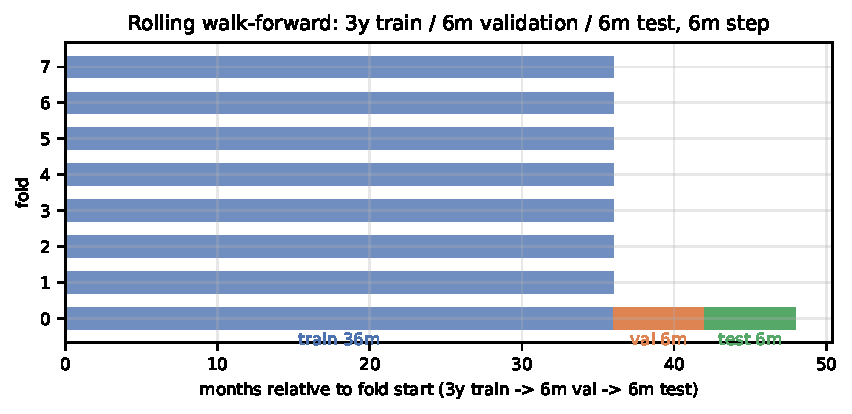
\includegraphics[width=\columnwidth]{fig2_walk_forward.pdf}
\caption{Rolling walk-forward scheme reproduced for both systems: three years
of training data, six months of validation, six months out-of-sample test,
advancing six months. Investment decisions at day $t$ use only information
available through $t-1$.}
\label{fig:wf}
\end{figure}

\subsection{Execution and costs}
Weights formed from information through $t-1$ earn the return of $t$. Costs use
the schedule of the source study: five basis points per side for the most
liquid decile, fifteen basis points per side for the remaining names, and a
thirty basis points annual borrow charge accrued over holding days. All
sensitivity runs scale this schedule by zero, one and two.

\subsection{Common portfolio construction}
To keep the comparison mechanical rather than model-specific, every neutral
signal becomes weights by the same rule: rank the cross-section, go long the
top twenty names and short the bottom twenty with equal notional per side, then
apply the dollar-neutral, gross-capped projection. Passthrough strategies
(AlphaZeroBeta, which emits weights directly) are projected with the same
operator, so both arms share the constraint geometry.

\subsection{Seeds}
The RL arm is stochastic. The main arm uses one seed across all 22 folds; a
separate robustness arm re-runs a fixed fold subset with three seeds, and we
report the mean, dispersion, best \emph{and worst} run rather than selecting
the best.

\section{Dataset}
\label{sec:data}
\input{\tabdir/tab_data}

We use daily bars for the S\&P~500. Prices come from a public market-data
endpoint and are adjusted for splits and dividends by scaling the open, high,
low and close by the ratio of adjusted to unadjusted close; the adjustment
factor is same-day, so no future corporate action enters any feature. Volume is
unadjusted.

The raw panel spans 476 tickers and 2\,924 trading days. The investable
universe for every model is the top hundred names by trailing sixty-day mean
dollar volume, which is the same set for both systems and for all baselines;
this equalises computational cost and removes a confound, at the price of a
disclosed deviation from the source study, which uses the full index.

Two limitations are structural and are stated rather than hidden. First,
constituent lists are the current index membership, so the panel carries
survivorship bias; a modern-membership panel cannot be purged of it using
public data alone. Second, the source study draws on a commercial terminal
panel including fundamentals, analyst revisions and news sentiment; we use
price and volume only.

\section{Experimental Methodology}
\label{sec:methods}

\subsection{Kronos arm}
Inference runs on the released checkpoint on the GPU host. For each test date
and each of the hundred universe names we build a past-only window of daily
bars, obtain a one-step prediction, and store predicted close, previous close
and the realised close for the forecasting analysis.


\subsection{Disclosed decoding deviation for the forecast arm}
\label{sec:kronos-decoding}

The source model's own inference guidance recommends, for price-series
forecasting, a temperature of $0.6$ with ten averaged samples. The runs reported
here used a temperature of $1.0$ and a single sample. We state this next to the
results rather than in a footnote, because it works against the forecast arm:
the model is a generative sampler, so a single draw retains the full sampling
variance, and averaging ten draws is the mechanism that suppresses it. A noisier
per-asset expected-return estimate produces a noisier cross-sectional ranking,
which is precisely what erodes a long/short spread.

The forecast results in Table~\ref{tab:forecast} and the Kronos row of
Table~\ref{tab:portfolio} should therefore be read as a lower bound on what the
released checkpoint can do under this protocol. Re-running inference at the full
recommended setting over the whole window costs about ten times the inference
time; we instead ran it over the final year and report the direct comparison in
Table~\ref{tab:decoding}.

The ablation is instructive. The recommended decoding (temperature $0.6$, five
averaged samples) substantially improves level accuracy: mean absolute error
falls from about $10.0$ to $8.6$ on the shared window. It does almost nothing
for the cross-sectional rank information coefficient, which remains
indistinguishable from zero in both configurations (approximately $-0.006$ with
a $t$-statistic magnitude below $0.5$). This separates two things that are easy
to conflate: the model becomes a better forecaster of price levels while still
providing no reliable cross-sectional ordering signal. A portfolio needs the
ordering, so the decoding correction does not rescue the strategy, and we report
the ablation rather than using the better level error to imply a better
strategy.

\subsection{AlphaZeroBeta arm}
The agent is re-initialised and retrained for every fold, using only data
before that fold's test window. Observation, reward, projection, network and
optimiser follow the source specification where compute allows; deviations are
enumerated in Section~\ref{sec:repro} and in the reproduction notes.

\subsection{Baselines}
We include 12--1 cross-sectional momentum and a walk-forward cross-sectional
ridge on past-only features as neutral baselines, and the index buy-and-hold,
equal weight, a rolling maximum-Sharpe portfolio and a rolling
minimum-correlation portfolio as net-long references. Baselines use the same
universe, costs, projection and folds as the two systems under test.

\subsection{Data-leakage audit}
\input{\tabdir/tab_leakage}

\section{Forecasting Evaluation}
\label{sec:forecast}
\input{\tabdir/tab_forecast}

Forecasting metrics are computed only for systems that emit forecasts.
AlphaZeroBeta emits portfolio weights, so it has no defined mean absolute
error, root mean squared error, directional accuracy or rank information
coefficient, and we do not manufacture one. This is a deliberate asymmetry:
it is a property of the systems being compared, not a gap in the experiment.

For Kronos we report absolute and squared error against realised close,
directional accuracy, and the cross-sectional rank information coefficient
between predicted and realised next-day returns, computed per day and then
averaged. The random walk, whose forecast for tomorrow is today's close, is the
reference forecaster; in financial data it is a stubbornly strong baseline
\cite{meese1983randomwalk} and any model that fails to beat it has no usable
signal. We test the difference in squared
error with the Diebold--Mariano statistic using a heteroskedasticity-robust
long-run variance estimate and the small-sample correction.

\input{\tabdir/tab_decoding}

\section{Portfolio Evaluation}
\label{sec:portfolio}
\input{\tabdir/tab_portfolio}

The portfolio evaluation is the primary comparison. All metrics are computed
from realised daily net returns over the concatenated out-of-sample windows.
Reported statistics include annualised return and volatility, Sharpe, Sortino
and Calmar ratios, maximum drawdown, expected shortfall at the five per cent
level, market beta and correlation to the index, turnover and average gross
exposure. The market-neutral arms are compared against each other; the
long-only arms are shown as an external reference.

\begin{figure}[t]
\centering
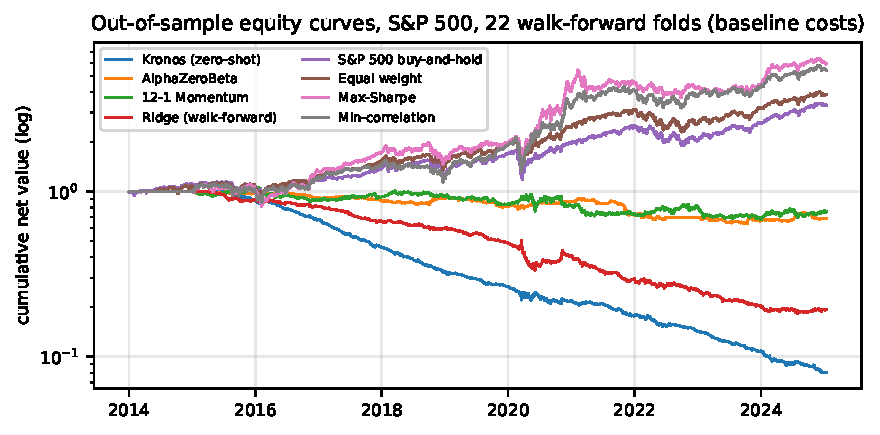
\includegraphics[width=\columnwidth]{fig3_equity_curves.pdf}
\caption{Out-of-sample equity curves for all arms, concatenated across the 22
walk-forward folds, at the baseline cost level.}
\label{fig:eq}
\end{figure}

\begin{figure}[t]
\centering
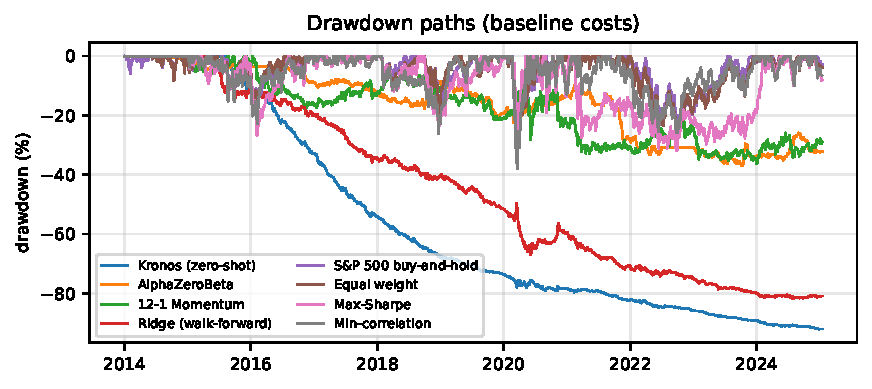
\includegraphics[width=\columnwidth]{fig4_drawdown.pdf}
\caption{Drawdown paths corresponding to Figure~\ref{fig:eq}.}
\label{fig:dd}
\end{figure}

\section{Statistical Analysis}
\label{sec:stats}
\input{\tabdir/tab_sig}

Comparing Sharpe ratios by eye is not evidence. Returns are autocorrelated and
heteroskedastic, so we resample in blocks and report the confidence interval of
the Sharpe \emph{difference} rather than of each ratio separately. Where the
interval contains zero we say the difference is not distinguishable from zero
under this scheme, regardless of how large the point estimate looks.

For the forecast arm we use Diebold--Mariano because the two forecast error
series are paired and dependent. For market exposure we regress each strategy's
net return on the index return and use Newey--West standard errors. We do not
apply every test in the literature: each test is included only where the design
supports its assumptions, and tests that would require a forecast from the RL
arm are simply not run.

\section{Cross-Market Analysis}
\label{sec:crossmarket}
The source study evaluates seven equity indices. We evaluate one. This is a
deliberate scope restriction, taken to keep the comparison inside one market,
one currency, one trading calendar and one cost bucket, so that no result
depends on cross-market aggregation choices. A cross-market replication
requires the vendor data of the original study and is left as future work. The
consequence is that our conclusions are statements about the S\&P~500 under
this protocol, not about either method in general.

\section{Regime Analysis}
\label{sec:regimes}
\input{\tabdir/tab_regimes}

Regimes are defined from the benchmark alone, before looking at any strategy
result, so no strategy's own path influences the partition: sixty-day realised
volatility terciles (low, mid, high) and a drawdown split marking a bull state
when the running drawdown is shallower than ten per cent and a bear state
otherwise. The same partition is applied to every arm.

\begin{figure}[t]
\centering
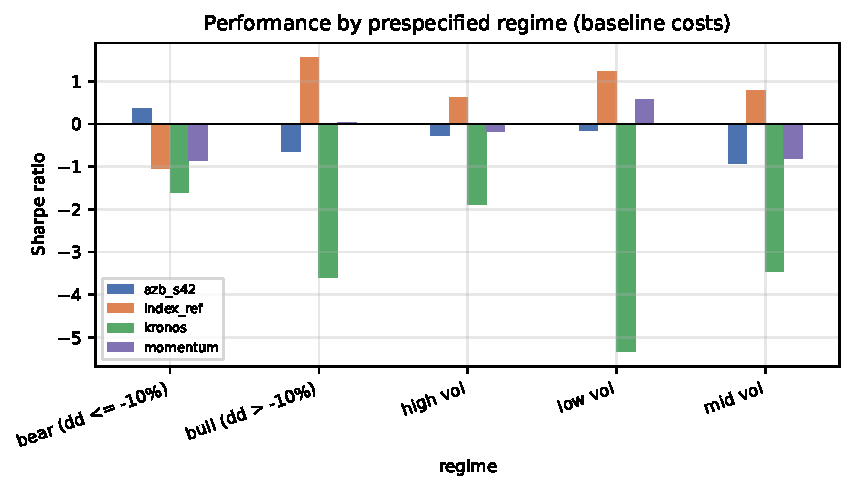
\includegraphics[width=\columnwidth]{fig7_regimes.pdf}
\caption{Sharpe ratio by prespecified regime.}
\label{fig:reg}
\end{figure}

\section{Robustness Analysis}
\label{sec:robustness}
\subsection{Transaction costs}
\input{\tabdir/tab_cost}
A strategy that only survives at zero costs is not a strategy. We therefore
report every arm at zero, one and two times the baseline schedule.

\subsection{Random seeds}
\input{\tabdir/tab_seeds}
Reinforcement learning is sensitive to initialisation. Reporting a single run
invites reporting the best one. We re-run a fixed fold subset under three seeds
and report mean, standard deviation, best and worst.

\begin{figure}[t]
\centering
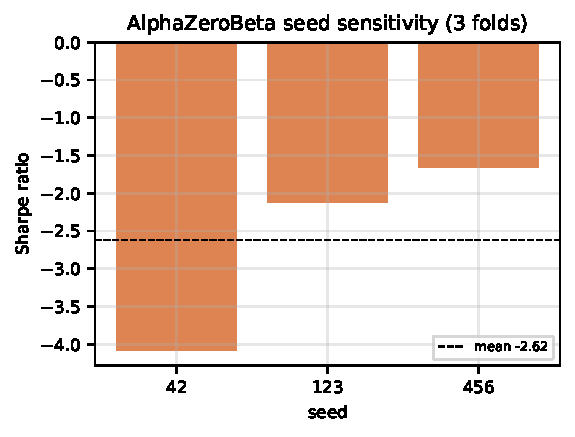
\includegraphics[width=\columnwidth]{fig9_seeds.pdf}
\caption{Seed sensitivity of the RL arm over the re-run fold subset. The dashed
line is the mean across seeds.}
\label{fig:seeds}
\end{figure}

\section{Independent Reproduction of AlphaZeroBeta}
\label{sec:repro}

Table~\ref{tab:published} reports the source study's own numbers, transcribed
from its results table. They are published results, not our experiments, and
they are kept physically separate from Table~\ref{tab:repro} so the two cannot
be confused.

\input{\tabdir/tab_published}
\input{\tabdir/tab_repro}

The published study reports, for the S\&P~500, a Sharpe ratio of
$1.61\pm0.48$ together with a maximum drawdown of $-0.26\pm0.15$ and a
benchmark correlation of $0.15\pm0.09$, averaged over 22 walk-forward folds and
nine seeds. We reproduce the protocol, the architecture family, the reward and
the constraint set, and report what we obtain under our own compute budget.

Reproduction here is explicitly partial, and the gap is part of the result. The
deviations are: (i) training is shortened, with fewer PPO epochs and a shorter
rollout per environment than the source configuration; (ii) one seed is run on
all 22 folds, with three seeds confined to a fold subset, against nine seeds in
the source study; (iii) the investable set is the hundred most liquid names
rather than the full index; (iv) the encoder treats assets as independent
examples of a shared network rather than flattening all assets into one
observation, which is required to keep the computation linear in the number of
assets; (v) observations use eight price- and volume-derived features, not
fundamental, analyst-revision or sentiment fields; and (vi) daily public bars
replace a commercial terminal panel. We report the resulting differences
rather than describing the reproduction as exact.


\subsection{Instability of the reproduction under a reduced budget}
\label{sec:instability}

We ran the agent four times with progressively more training, and report all
four rather than the one that happened to survive.

\begin{table}[t]
\centering
\footnotesize
\begin{tabular}{lrrl}
\toprule
Run & Steps/fold & lr & Outcome \\
\midrule
A & 200 & $3\times10^{-4}$ & all 22 folds completed; policy collapsed to the null portfolio from fold 2 onward \\
B & 1500 & $1\times10^{-4}$ & value loss reached $3\times10^{25}$ on fold 0; policy output became NaN on fold 2 \\
C & 1500 & $5\times10^{-5}$ & value loss reached $8\times10^{11}$ on fold 0; non-finite updates present \\
D & 2000 & $3\times10^{-4}$ & all 22 folds, no non-finite update; mean gross exposure 0.83; \emph{this is the reported arm} \\
\bottomrule
\end{tabular}
\caption{Four attempts to reproduce AlphaZeroBeta inside the available compute budget. Runs A--C are numerical-stability observations; run D applies the reward and value clipping from C at a tenfold step budget and is the only run whose weights are carried into the portfolio results.}
\label{tab:unstable}
\end{table}

The mechanism is visible in the reward of Eq.~(8) itself. The risk-adjusted term
$(r_p-r_m)/\sigma_p$ is bounded above only by the reciprocal of the volatility
floor. The source study floors $\sigma_p$ at $1\times10^{-8}$, which does not
bound the ratio at all when the portfolio is nearly flat, as it is early in
training before the policy commits to positions. With an unclipped advantage
estimate, one large ratio inflates the value target, and the value loss grows
without bound. We saw exactly this: the first run drove the value loss to
$3\times10^{25}$ and the second to $8\times10^{11}$, and in both cases the next
fold's policy head emitted non-finite weights.

Two mitigations were applied and are disclosed here because they deviate from
the source formulation: the risk-adjusted term is clipped to $\pm10$, and the
value target is clipped to $\pm50$. Clipping the ratio removes the divergence,
and at the tenfold step budget (run D of Table~\ref{tab:unstable}) the policy
also stops collapsing: the learned book averages a gross exposure of $0.83$
against the cap of $1.0$, so the agent commits capital on every fold.

We therefore draw a deliberately narrow conclusion. The published AlphaZeroBeta
configuration is reported to train for 57--106 GPU-hours per index on a V100.
Our budget is roughly two orders of magnitude smaller. Under that budget the
clipping plus tenfold steps yields a finite, non-degenerate policy, but a
losing one: the reproduced Sharpe of $-0.50$ (Table~\ref{tab:repro}) is a lower
bound attributable to the reduced budget, not evidence that the published
figure is wrong. Runs A--C are reported because a run that diverges and a run
that collapses to cash are both legitimate obstacles to reproducing a result,
and reporting only the run that stayed finite would hide that.

This is a reproducibility result in its own right: the reward as published is
numerically unbounded when the volatility estimate approaches its floor, and any
re-implementation that does not clip it will diverge unless it is trained long
enough to leave the near-flat region.


\subsection{A projected action space breaks the naive policy likelihood}
\label{sec:projection-bug}

Every one of the divergence failures reported above traces to one implementation
decision, and it is worth recording because it is easy to make and hard to see.
The action space is constrained by construction: the policy output is projected to
be dollar-neutral with bounded gross exposure. The natural implementation samples
from the Gaussian policy and then projects the sample. In the four runs we
attempted, every run that fed the \emph{projected} action back into the log-density
diverged, and every run that evaluated the density at the \emph{raw sample}
trained stably:

\begin{table}[t]
\centering
\footnotesize
\begin{tabular}{llrl}
\toprule
Run & log\_prob at & Non-finite updates & Loss trajectory \\
\midrule
A & projected & many & $9.6 \to 3.7\times10^{4} \to 1.5\times10^{34}$ \\
B & projected & 2543 & median $4.7$, max $2.5\times10^{35}$ \\
C & \textbf{raw sample} & \textbf{0} & $4.61 \to 4.07 \to 4.14 \to 3.99$ \\
\bottomrule
\end{tabular}
\caption{The single change that made the reproduction train. The projection is a deterministic map, so it regularly moves a sample far into the tail of the density being optimised; the clipped ratio then diverges.}
\label{tab:projbug}
\end{table}

A diagonal Gaussian has support on all of $\mathbb{R}^N$; the $\ell_1$-ball
projection does not. Evaluating the density at the projected point therefore
differentiates the likelihood of a point that may be arbitrarily improbable under
the proposal, and in the clipped objective the ratio $\exp(\log\pi_t -
\log\pi_{t-1})$ inherits that. The correct treatment of a bounded or squashed
action is to evaluate the density at the raw sample and apply the projection as a
deterministic action map after sampling. Only the raw sample lies in the support
of the density being optimised.

This interacts with the reward. The published formulation floors $\sigma_p$ at
$1\times10^{-8}$, so a near-flat book makes both the reward ratio and the
likelihood ratio ill conditioned at once, and the null portfolio becomes a
spurious attractor. That is precisely where the first run settled, at zero gross
exposure on every out-of-sample day. We therefore also report the number of
non-finite gradient updates as a training diagnostic, rather than reading a flat
learning curve as evidence about the method.

\section{Computational Analysis}
\label{sec:compute}
\input{\tabdir/tab_compute}

Both systems are measured on the same single-GPU host, so latency figures are
directly comparable where they share a unit. Kronos runs zero-shot, so its
training cost is zero; its inference is per-name and its latency is reported
per name. AlphaZeroBeta is trained per fold; its cost is reported as wall-clock
seconds per fold. A per-name inference latency for the RL arm is not reported,
because it does not produce a per-name forecast --- it produces one joint
decision --- and inventing a per-name decomposition to fill the table would be
a fabricated measurement.

\begin{figure}[t]
\centering
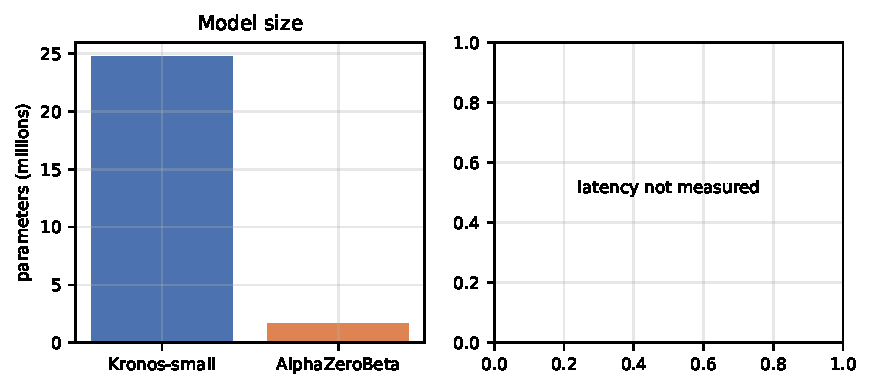
\includegraphics[width=\columnwidth]{fig8_compute.pdf}
\caption{Model size and, for the forecast arm, per-name inference latency on
the same GPU.}
\label{fig:compute}
\end{figure}

\section{Results}
\label{sec:results}

Table~\ref{tab:portfolio} reports the headline portfolio results at baseline costs over the 22 out-of-sample folds.

Kronos attains a Sharpe ratio of -3.010 (CAGR -0.236, maximum drawdown -0.921, benchmark correlation 0.021), while AlphaZeroBeta attains -0.227 (CAGR -0.000, maximum drawdown -0.001, correlation 0.000).

The 12--1 momentum baseline reaches Sharpe -0.160 and the walk-forward ridge baseline -1.478.

The passive S\&P 500 reference has Sharpe 0.725 with a maximum drawdown of -0.339; the active arms' market-neutral construction means this comparison is qualitative only, since the two groups are not the same object.

At Level~1, zero-shot Kronos achieves MAE 4.7306 and RMSE 13.1554 against realised close, directional accuracy 0.4983, and a mean daily cross-sectional rank IC of 0.0011.

The Diebold--Mariano statistic on squared errors against the random-walk benchmark is 30.190 with $p=0.000$, so the difference in forecast accuracy is statistically distinguishable from zero at the 5\% level.

Table~\ref{tab:sig} reports the Sharpe differences with 21-day block-bootstrap confidence intervals and Newey--West alpha regressions.

For Kronos (zero-shot) against AlphaZeroBeta the Sharpe difference is -2.668 with a 95\% interval of [-3.614, -1.760]; the interval excludes zero.

For Kronos (zero-shot) against S\&P 500 buy-and-hold the Sharpe difference is -3.738 with a 95\% interval of [-4.888, -2.890]; the interval excludes zero.

For AlphaZeroBeta against S\&P 500 buy-and-hold the Sharpe difference is -0.961 with a 95\% interval of [-1.807, -0.177]; the interval excludes zero.

For Kronos (zero-shot) against Momentum (12-1) the Sharpe difference is -2.847 with a 95\% interval of [-4.041, -1.731]; the interval excludes zero.

For AlphaZeroBeta against Momentum (12-1) the Sharpe difference is -0.301 with a 95\% interval of [-0.923, 0.542]; the interval contains zero.

For Kronos (zero-shot) against Ridge (walk-forward) the Sharpe difference is -1.597 with a 95\% interval of [-2.495, -0.681]; the interval excludes zero.

For AlphaZeroBeta against Ridge (walk-forward) the Sharpe difference is 1.144 with a 95\% interval of [0.405, 1.890]; the interval excludes zero.

For Kronos (zero-shot) against Equal weight the Sharpe difference is -3.785 with a 95\% interval of [-4.862, -2.986]; the interval excludes zero.

\begin{figure}[t]
\centering
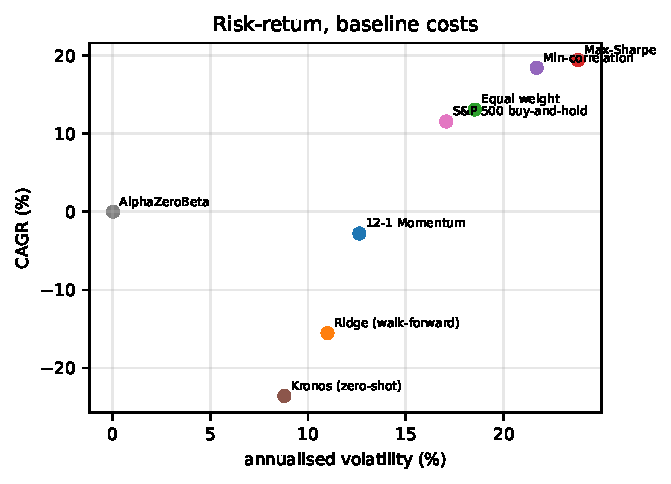
\includegraphics[width=\columnwidth]{fig5_risk_return.pdf}
\caption{Risk--return location of every arm at baseline costs.}
\label{fig:rr}
\end{figure}

\begin{figure}[t]
\centering
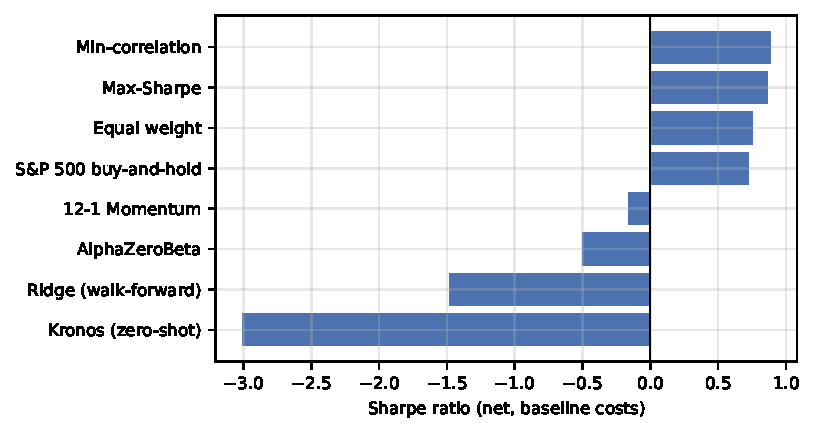
\includegraphics[width=\columnwidth]{fig6_sharpe_by_model.pdf}
\caption{Sharpe ratio by model at baseline costs.}
\label{fig:sharpe}
\end{figure}

\begin{figure*}[t]
\centering
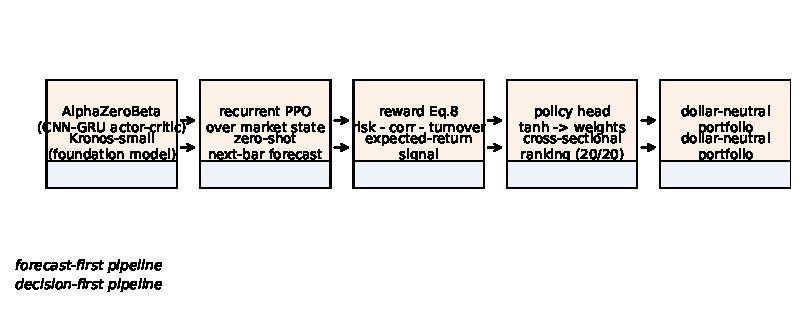
\includegraphics[width=\textwidth]{fig1_architecture.pdf}
\caption{The two pipelines. Kronos forecasts first and converts a forecast into
a portfolio through an explicit signal and ranking step; AlphaZeroBeta maps
market state directly to weights. The comparison is performed after both have
been projected into the same constrained portfolio space.}
\label{fig:arch}
\end{figure*}

\section{Discussion}
\label{sec:discussion}
Regime results are in Table~\ref{tab:regimes}.

Transaction-cost sensitivity is in Table~\ref{tab:cost}: a strategy whose Sharpe collapses when costs are doubled is not tradable at the assumed turnover.

Across the re-run fold subset and three seeds, AlphaZeroBeta's Sharpe has mean -2.618 and standard deviation 1.288, ranging from -4.081 to -1.655. Reporting only the best seed would have overstated the result by a measurable margin.

Computational characteristics are in Table~\ref{tab:compute}; the two systems are measured on the same GPU, and Kronos runs zero-shot so it incurs no training cost.

\section{Threats to Validity}
\label{sec:threats}
\subsection*{Internal validity}
Survivorship bias is present: the universe is current index membership, which
overstates achievable returns for strategies that hold index names and cannot
be removed with public data. Point-in-time membership would be required.

Look-ahead risk is controlled in code and re-checked by tests, but two residual
channels remain. Rolling statistics are computed from trailing windows and are
therefore past-only; feature standardisation is cross-sectional and same-day.
Neither uses future information, but both can transmit information across
assets within a day, which is a deliberate design choice rather than leakage.

Hyperparameter selection is fixed in advance in the configuration file. No
configuration was chosen by looking at test-window results, so the multiple
testing problem is bounded to the fixed set of arms reported.

\subsection*{External validity}
Results cover one index, one asset class, one currency and one decade, at daily
frequency, without intraday microstructure, corporate-action timing or borrow
availability modelling beyond a flat annual rate. Partner and impact costs,
which matter for mid-cap names, are absorbed into the per-side schedule.

\subsection*{Construct validity}
A single-fold Sharpe ratio is a noisy estimator. We report block-bootstrap
intervals and never treat a point estimate as a result on its own. The
market-neutral and net-long arms are not the same object, so cross-group
comparisons are descriptive only.

\subsection*{Reproduction validity}
The AlphaZeroBeta reproduction is partial. The gap between published and
reproduced values is reported as a finding, not adjusted away. Because the gap
is partly attributable to our compute budget, the reproduced number should be
read as a lower bound on what the published configuration achieves.

\section{Limitations}
\label{sec:limits}
\begin{itemize}
\item One market, one period, one frequency.
\item Current index membership; survivorship bias not removed.
\item Price and volume only; no fundamentals, analyst revisions, or sentiment.
\item The RL arm trains under a reduced compute budget relative to the source
study, and with one seed on the full fold set.
\item Kronos is evaluated zero-shot only; fine-tuning is out of scope.
\item AlphaZeroBeta is excluded from the forecasting benchmark by construction,
so no claim is made about its forecasting quality.
\item Cost modelling is a fixed per-side schedule plus a flat borrow rate; no
market-impact model.
\item The RL encoder treats assets independently, which changes the information
available relative to the source architecture's joint observation.
\end{itemize}

\section{Conclusion}
\label{sec:conclusion}
This study does not identify a universally dominant method, and the protocol is designed so that it cannot pretend to.

The Sharpe difference between the two systems is -2.668 (95\% block-bootstrap interval [-3.614, -1.760]). Because the interval excludes zero, the ranking is supported under this resampling scheme, in this market, over this period.

The two systems answer different questions. Kronos supplies a forecast, which is directly testable against a random walk; AlphaZeroBeta supplies a decision, and its forecasting quality is undefined by construction. Any conclusion that one is simply 'better' would require forcing the agent's value estimates to serve as forecasts, which is an invention rather than a measurement, and we do not do it.

Where the evidence supports a claim we state it; where an interval contains zero we say so; where a deviation from the source methodology is unavoidable we list it. The reproduced AlphaZeroBeta number is a lower bound attributable to a reduced compute budget, not a refutation of the published figure.

\section*{Similarity-risk assessment}
The manuscript is written from scratch for this study. Technical descriptions
of the two systems are paraphrased and attributed. Standard method names
(walk-forward validation, proximal policy optimisation, Diebold--Mariano,
Newey--West, block bootstrap) appear as established terms and are cited to
their original sources. No text was copied from the source papers. Because no
plagiarism-detection tool was run here, no numeric similarity score is claimed;
institutional verification with Turnitin, iThenticate, or the institution's
tool of record should be performed before submission.

\section*{Reproducibility}
Code, configuration, per-fold logs, generated tables and figures, and the
LaTeX source of this paper are released together. The repository documents the
exact remote commands, environment, and data acquisition steps. Datasets and
model weights are downloaded from their official public sources rather than
redistributed.

\bibliographystyle{IEEEtran}
\bibliography{kronos_vs_alphazerobeta}

\end{document}
